\documentclass[10pt, spanish, pdftex]{../.template/template}

%%%%%%%%%%%%%%%%%%%%%%%%%%%%%%%%%%%%%%%%%%%%%%%%%%%%%%%%
%               UC3M Work report template              %
%           Universidad Carlos III de Madrid           %
%              Author: Aitor Alonso Núñez              %
%              Last update: March 8, 2018              %
%%%%%%%%%%%%%%%%%%%%%%%%%%%%%%%%%%%%%%%%%%%%%%%%%%%%%%%%

%%%%% Preamble %%%%%
\usepackage{fancyhdr}				% To add header and footer
\usepackage{graphicx}				% To add images
\usepackage{caption}				% To add captions
\usepackage{subcaption}				% To add subcaptions
\usepackage{lipsum}					% Example Lorem ipsum text
\usepackage[hidelinks]{hyperref}	% Index elements works as cross references. Also functional links to internet pages
\usepackage{nameref}				% Allow to add labels with \label{name} which can be reference with \nameref{name}
\author{Aitor Alonso Núñez}			% This is me!

\usepackage{listings}
\graphicspath{{images/}}
\usepackage[table,xcdraw]{xcolor}

\newcommand*{\namerefs}[1]{\textit{\underline{\color{uc3mNewBlue}\nameref{#1}}}}

%%%%% Coauthors info %%%%%
%%[1-2] If you want to show coauthors email address on the title page, enable \emailtrue. Otherwise, enable \emailfalse
\emailtrue
% \emailfalse
%% If coauthors are between 1 and 2 uncomment these options. Comment it otherwise.
%% You can leave empty keys {} if you need to.
\coauthorstwotrue		% coauthors two = true
\coauthorsthreefalse	% coauthors three = false
\coauthorsfourfalse		% coauthors four = false
\coauthorstwo{Aitor Alonso Núñez}{NIA 100346169}{Gr. 83}{Daniel Gak Anagrov}{NIA 100318133}{Gr. 83}
%%[3] If you enabled \emailtrue, uncomment the option below
\emailstwo{100346169@alumnos.uc3m.es}{100318133@alumnos.uc3m.es}

%% If coauthors are between 1 and 2 uncomment these options. Comment it otherwise.
%% You can leave empty keys {} if you need to.
% \coauthorstwofalse		% coauthors two = false
% \coauthorsthreetrue		% coauthors three = true
% \coauthorsfourfalse		% coauthors four = false
% \coauthorsthree{Name1 Lastname1}{NIA 100XXXXXX}{Gr. XX}{Name2 Lastname2}{NIA 100XXXXXX}{Gr. XX}{Name3 Lastname3}{NIA 100XXXXXX}{Gr. XX}
%% If you want to show on the title page the email address of these coauthors uncomment the next options
%% and comment \emailfalse. In other case, comment everything except \emailfalse
% \emailsthree{email1@domain.tld}{email2@domain.tld}{email3@domain.tld}

%%[4] If coauthors are between 1 and 2 uncomment these options. Comment it otherwise.
%% You can leave empty keys {} if you need to.
% \coauthorstwofalse		% coauthors two = false
% \coauthorsthreefalse		% coauthors three = false
% \coauthorsfourtrue		% coauthors four = true
% \coauthorsfour{Name1 Lastname1}{NIA 100XXXXXX}{Name2 Lastname2}{NIA 100XXXXXX}{Name3 Lastname3}{NIA 100XXXXXX}{Name4 Lastname4}{NIA 100XXXXXX}
%% If you want to show on the title page the email address of these coauthors uncomment the next options
%% and comment \emailfalse. In other case, comment everything except \emailfalse
% \emailsfour{email1@domain.tld}{email2@domain.tld}{email3@domain.tld}{email4@domain.tld}


%%%%% Basic data about the document (Degree, subject, title, campus, page number custom text) %%%%%
\documentdata{Grado en Ingeniería Informática}{Aprendizaje Automático}{Práctica 3\\Aprendizaje por refuerzo}{Escuela Politécnica Superior}{Página }

%%%%% Page style %%%%%
\header
\footer
\pagestyle{fancy}
\begin{document}

%%%%% Page title %%%%%
\titleMain

%%%%% Index %%%%%
\tableofcontents 	% We add the index
\newpage 			% And before index we start on a new page

%%%%% CONTENIDO DEL DOCUMENTO %%%%%
%% VERY IMPORTANT!!! On the first line of this .tex file, select Spanish or English language to coincide with document text language
\section{Introducción}
    \p{Este documento sirve como memoria de la práctica 3: \textit{Aprendizaje por refuerzo}, de la asignatura Aprendizaje Automático. En la misma, hemos tenido que programar un agente que juegue de forma automática a Mario haciendo uso del algoritmo de aprendizaje por refuerzo \textit{Q-learning}, de forma que el dominio ha quedado representado como un espacio de estados discretos, identificando y evaluando diferentes situaciones para obtener una política de actuación a partir de este algoritmo.}
    \p{A lo largo del presente documento se describirán los siguientes puntos, en el mismo orden que como se ha realizado en esta práctica:}
    \begin{itemize}
        \item \namerefs{td}: Este apartado contiene la toma de ejemplos, la descripción de los atributos, la forma de almacenarlos y el preprocesamiento aplicado.
        \item \namerefs{is}: Explica el critero de creación de situaciones y la forma en la que se identifica si un tick (instancia de un momento de juego) pertenece a ella o no.
        \item \namerefs{ql}: En este apartado queda recogido el cálculo del refuerzo y la aplicación del algoritmo de aprendizaje por refuerzo \textit{Q-Learning}.
        \item  Al final de este documento quedan recogidos la \namerefs{e}, la \namerefs{dme}, y las \namerefs{c} y \namerefs{cp}
    \end{itemize}


\section{Tratamiento de datos}\label{td}


    \subsection{Atributos}\label{a} % Descripción y rango de valores
    \p{Nuestras instancias de entrenamiento, que han sido tomadas con el agente humano \texttt{P3HumanAgent} con ayuda del
    código de toma de datos contenido en el fichero \texttt{tools/TrainingFile.java}, generan una tupla de datos por cada tick de la ejecución del juego que contiene la siguiente información:}
    \begin{itemize}
        \item Atributos del tick $N$.
        \item Acción ejecutada en el tick $N$.
        \item Atributos del tick $N+12$.
        \item Refuerzo (cálculo inicial en tiempo de toma de ejemplos finalmente ignorado, ver \namerefs{refuerzo}).
    \end{itemize}
    \p{Todas estas tuplas han sido escritas en el fichero \texttt{weka/ejemplos\_entrenamiento/P3HumanAgent\_1.arff} con una cabecera apropiada para su tratamiento con Weka. A continuación se describen los atributos de los que constan estas tuplas.}
    \newpage

    \subsubsection{Atributos para ayudar a localizar o identificar la instancia de entrenamiento}
    \begin{enumerate}
        \item \textbf{timeSpent:} Tiempo gastado en segundos del juego (\texttt{short})
        \item \textbf{timeLeft:} Tiempo restante en segundos del juego (\texttt{short})
    \end{enumerate}
    \subsubsection{Atributos relacionados con la intermediateReward}
    \begin{enumerate}
        \setcounter{enumi}{2}
        \item \textbf{intermediateReward:} Recompensa actual en el momento de la captura de la instancia (\texttt{short})
        \item \textbf{intermediateRewardWonLastTick:} Recompensa obtenida respecto al tick anterior (1/24s) (\texttt{short})
        \item \textbf{intermediateRewardWonLast6Ticks:} Recompensa obtenida respecto a los 6 ticks anteriores (1/4s) (\texttt{short})
        \item \textbf{intermediaRewardWonFuture6Ticks:} Recompensa obtenida 6 ticks después (1/4s) de ejecutar la acción de esta instancia (\texttt{short}). Este atributo no existe para la instancia del tick $N+12$ (segunda mitad de la tupla).
    \end{enumerate}
    \subsubsection{Atributos relacionados con la matriz de observación (mergeObs)}
    \begin{enumerate}
        \setcounter{enumi}{6}
        \item \textbf{nearestEnemyLeftDistance:} Distancia euclídea al enemigo más cercano a la izquierda de Mario (\texttt{float})
        \item \textbf{nearestEnemyLeft\_X:} posición X de la mergeObs del enemigo más cercano por la izquierda (\texttt{byte})
        \item \textbf{nearestEnemyLeft\_Y:} posición Y de la mergeObs del enemigo más cercano por la izquierda (\texttt{byte})
        \item \textbf{nearestEnemyRightDistance:} Distancia euclídea al enemigo más cercano a la derecha de Mario (\texttt{float})
        \item \textbf{nearestEnemyRight\_X:} posición X de la mergeObs del enemigo más cercano por la derecha (\texttt{byte})
        \item \textbf{nearestEnemyRight\_Y:} posición Y de la mergeObs del enemigo más cercano por la derecha (\texttt{byte})
        \item \textbf{nearestBlockLeftDistance:} Distancia euclídea al bloque más cercano a la izquierda de Mario (\texttt{float})
        \item \textbf{nearestBlockLeft\_X:} posición X de la mergeObs del bloque más cercano por la izquierda (\texttt{byte})
        \item \textbf{nearestBlockLeft\_Y:} posición Y de la mergeObs del bloque más cercano por la izquierda (\texttt{byte})
        \item \textbf{nearestBlockRightDistance:} Distancia euclídea al bloque más cercano a la derecha de Mario (\texttt{float})
        \item \textbf{nearestBlockRight\_X:} posición X de la mergeObs del bloque más cercano por la derecha (\texttt{byte})
        \item \textbf{nearestBlockRight\_Y:} posición Y de la mergeObs del bloque más cercano por la derecha (\texttt{byte})
        \item \textbf{nearestCoinLeftDistance:} Distancia euclídea a la moneda más cercana a la izquierda de Mario (\texttt{float})
        \item \textbf{nearestCoinLeft\_X:} posición X de la mergeObs de la moneda más cercana por la izquierda (\texttt{byte})
        \item \textbf{nearestCoinLeft\_Y:} posición Y de la mergeObs de la moneda más cercana por la izquierda (\texttt{byte})
        \item \textbf{nearestCoinRightDistance:} Distancia euclídea a la moneda más cercana a la derecha de Mario (\texttt{float})
        \item \textbf{nearestCoinRight\_X:} posición X de la mergeObs de la moneda más cercana por la derecha (\texttt{byte})
        \item \textbf{nearestCoinRight\_Y:} posición Y de la mergeObs de la moneda más cercana por la derecha (\texttt{byte})
        \item \textbf{numEnemiesObserved:} número total de enemigos identificados en la matriz de observación (\texttt{short})
        \item \textbf{numCoinsObserved:} número total de monedas identificadas en la matriz de observación (\texttt{short})
    \end{enumerate}
    \subsubsection{Atributos booleanos o binarios}
    \begin{enumerate}
        \setcounter{enumi}{26}
        \item \textbf{enemyNearRight:} valor numérico binario (0-1) que indica si hay (1) o no (0) enemigos en una submatriz de la matriz de observación ([fil][col] == [8-9][10-11]) (\texttt{byte})
        \item \textbf{blockNearRight:} valor numérico binario (0-1) que indica si hay (1) o no (0) obstáculos en una submatriz de la matriz de observación ([fil][col] == [8-9][10-11]) (\texttt{byte})
        \item \textbf{enemyAheadOnFloorHeight:} valor numérico binario (0-1) que indica si hay (1) o no (0) enemigos en una submatriz de la matriz de observación ([fil][col] == [10][10-11]) (\texttt{byte})
        \item \textbf{blockAheadOnFloorHeight:} valor numérico binario (0-1) que indica si hay (1) o no (0) obstáculos en una submatriz de la matriz de observación ([fil][col] == [10][10-11]) (\texttt{byte})
        \item \textbf{abyssAhead:} valor numérico binario (0-1) que indica si hay (1) o no (0) foso/abismo/acantilado delante (en matriz de observación [16][10] no hay bloque) (\texttt{byte})
        \item \textbf{isMarioOnGround:} valor numérico binario (0-1) que indica si Mario está (1) o no está (0) en el suelo (\texttt{byte})
        \item \textbf{isMarioAbleToJump:} valor numérico binario (0-1) que indica si Mario puede (1) o no puede (0) saltar (bloqueo de salto) (\texttt{byte})
        \item \textbf{isMarioAbleToShoot:} valor numérico binario (0-1) que indica si Mario puede (1) o no puede (0) disparar (\texttt{byte})
        \item \textbf{isMarioCarrying:} valor numérico binario (0-1) que indica si Mario está (1) o no está (0) llevando un caparazón (\texttt{byte})
        \item \textbf{enemyWasKilledBin:} valor numérico binario (0-1) que indica si ha muerto (1) o no (0) un enemigo en la instancia actual (\texttt{byte})
        \item \textbf{marioWasInjuredBin:} valor numérico binario (0-1) que indica si Mario ha sido herido (1) o no (0) en la instancia actual (\texttt{byte})
        \item \textbf{isSlopeDown:} valor numérico binario (0-1) que indica si hay (1) o no (0) un desnivel delante (en columna [10]) (\texttt{byte})
    \end{enumerate}
    \subsubsection{Otros atributos}
    \begin{enumerate}
        \setcounter{enumi}{38}
        \item \textbf{coinsGainedLastTick:} número de monedas conseguidas respecto al tick anterior (\texttt{byte})
        \item \textbf{marioMode:} modo actual de Mario: 0,1,2 == pequeño, grande, fuego (\texttt{byte})
        \item \textbf{marioStatus:} estado actual de Mario: 0,1,2 == muerto/derrota, victoria, corriendo/jugando (\texttt{byte})
    \end{enumerate}
    
    \subsubsection{Acción realizada}\label{acciones}
        \textbf{ActionKey} es el atributo que contiene acción o acciones realizadas durante esta instancia, codificada como un valor numérico que diferencia varias situaciones (\texttt{byte})
        \begin{enumerate}
            \setcounter{enumi}{-1}
            \item Ninguna acción o tecla pulsada: \textbf{0}
            \item Salto (tecla A): \textbf{1}
            \item Derecha (tecla flecha derecha): \textbf{2}
            \item Derecha-salto (teclas flecha derecha + A): \textbf{3}
            \item Derecha-disparar (teclas flecha derecha + S): \textbf{4}
            \item Derecha-salto-disparar (teclas flecha derecha + A + S): \textbf{5}
            \item Izquierda (tecla flecha izquierda): \textbf{6}
            \item Izquierda-salto (teclas flecha izquierda + A): \textbf{7}
            \item Izquierda-disparar (teclas flecha izquierda + S): \textbf{8}
            \item Izquierda-salto-disparar (teclas flecha izquierda + A + S): \textbf{9}
        \end{enumerate}
        \p{Como se puede observar, el tipo de cada atributo se ha elegido buscando ocupar la menor memoria posible, dado que el tipo de agente a programar hace un uso intensivo de memoria principal (aunque no tanto como el agente de la práctica anterior, \textit{P2: Aprendizaje basado en instancias}).}
    
        \subsubsection{Refuerzo}
        \p{Inicialmente se incluyó el refuerzo en la toma de ejemplos, como atributo final de las tuplas. Este esfuerzo ha sido finalmente ignorado puesto que hemos comprobado en la experimentación y evaluación del agente que la forma en la que lo calculamos originalmente no fue la más acertada. Esta primera aproximación se calculaba de la forma:}\\\\
        $(intermediateReward\_tickN12 + positionX\_tickN12) - (intermediateReward\_tickN + positionX\_tickN)$
        \p{Para más información sobre como calculamos finalmente el refuerzo, revise la sección \namerefs{refuerzo}.}
    
    \subsection{Toma de ejemplos}\label{tde}

    \p{Para la toma de ejemplos hemos utilizado tanto el agente humano \texttt{P3HumanAgent}, como el agente bot proporcionado \texttt{BaseLine}.}

    \p{El comportamiento humano, en este contexto, realiza acciones que tienen un objetivo constante a lo largo de la partida, no obstante, el humano no es una máquina perfecta y en situaciones idénticas es capaz de tomar acciones distintas, ya que en este contexto su comportamiento es más estocástico que otros bots implementados.}
    \p{Por esta misma razón, las instancias contendrán variedad de acciones ejecutadas para situaciones similares para las que se ha obntenido distinto refuerzo, y será la tarea del algoritmo de aprendizaje por refuerzo Q-Learning identificar los Q-Valores que determinan que acción es la mejor en cada situación.}

    \p{En cuanto al comportamiento del bot \texttt{BaseLine}, completamente estocástico, nos proporciona multitud de instancias de entrenamiento muy distintas unas a las otras para situaciones muy similares, lo que por los mismos motivos indicados anteriormente, serán fácilmente aprovechables en el algoritmo Q-Learning. Asimismo, el uso del bot nos permite tomar ejemplos con más rapidez que el agente humano.}

    \p{Por ello, centraremos nuestros esfuerzos en la parametrización y el cálculo del refuerzo incluido en las tuplas (estado actual,acción,estado siguiente) del algoritmo Q-Learning para crear nuestro Agente.}

\section{Identificación de situaciones}\label{is}

    \p{Como bien se ha comentado anteriormente, las tuplas de datos quedan almacenadas en un fichero \texttt{.arff} manipulable con Weka, para que se pueda utilizar esta herramienta para ffiltrar los datos y determinar las diferentes situaciones sin introducir conocimiento del dominio del juego.}
    \p{Inicialmente se ha utilizado el algoritmo \texttt{K-medias} para determinar las situaciones o estados de nuestro agente, ya que es un algoritmo de clustering sencillo y no supervisado, estudiado en las sesiones de teoría, y que nos proporciona unos centroides contra los que comparar posteriormente y con facilidad tanto las instancias de entrenamiento como las instancias del juego durante la ejecución del agente, con el fin de identificar la fila de la tabla Q sobre la que actuar.}
    \p{A continuación se explica el tratamiento de los datos previo a su clusterización con Weka. Posteriormente se explicarán otros métodos utilizados para la identificación de situaciones y la implementación final.}
    
    \subsection{Borrado de atributos}
        \p{Las tuplas de datos que disponemos contienen atributos contraproducentes para generar cluster sobre ellos, por lo que en primer lugar, se ha realizado un borrado de atributos antes de calcular los clusters. De esta forma se han eliminado todas los atributos del tick $N+12$, la acción realizada así como los siguiente atributos irrelevantes del tick $N$:}
        \begin{itemize}
            \item timeSpent
            \item timeLeft
            \item enemyWasKilledBin
            \item marioWasInjuredBin
            \item coinsGainedLastTick
            \item marioMode
            \item marioStatus
        \end{itemize}
        \p{Estos atributos se han considerado despreciables puesto que no ofrecen información relevante para determinar el comportamiento de mario en el tick actual, por lo que solo serán un inconveniente para determinar los clusters.}

    \subsection{Identificación con clustering (K-medias)}
        \p{Este algoritmo toma \texttt{K} como parámetro principal, el cual especifica el número de clusters a formar. Con ello, obtenemos \texttt{K} centroides que son representaciones medias de una instancia ideal. De esta forma se ha realizado una experimentación de diferentes número de clusters, para $K=5$, $K=10$ y $K=20$, obteniendo resultados en el comportamiento del agente muy similares para los distintos valores de K con la misma parametrización del algoritmo Q-Learning.}
        \p{Esto nos ha hecho pensar que el uso de técnicas de clustering no era lo más adecuado en este dominio. Finalmente, hemos procedido a una interpretación de las situaciones a mano, siguiendo las indicaciones dadas por Jose Carlos en clase, para lo que hemos implementado un clasificador manual en forma de árbol \texttt{if-else}.}

    \subsection{Identificación manual (árbol \texttt{if-else})}\label{ifelse}
        \p{Se ha implementado un clasificador manual (sin ayuda de ninguna técnica de aprendizaje automático) en forma de árbol \texttt{if-else} para clasificar las instancias en 16 situaciones diferentes. Nos hemos centrado en clasificar las instancias basándonos en si Mario está o no en el aire, si hay enemigos cerca, y si hay obstáculos cerca; en este orden de prioridad. Esto ha dado lugar a las siguientes situaciones:}
        \begin{enumerate}
            \setcounter{enumi}{-1}
                \item Mario está \textbf{en el aire}, hay \textbf{enemigo} y \textbf{obstáculo} cerca, y \textbf{ambos} están \textbf{a la misma altura} que Mario.
                \item Mario está \textbf{en el aire}, hay \textbf{enemigo} y \textbf{obstáculo} cerca, y el \textbf{enemigo} está \textbf{a la misma altura} que Mario.
                \item Mario está \textbf{en el aire}, hay \textbf{enemigo} y \textbf{obstáculo} cerca, y el \textbf{obstáculo} está \textbf{a la misma altura} que Mario.
                \item Mario está \textbf{en el aire}, hay \textbf{enemigo} y \textbf{obstáculo} cerca, y \textbf{ambos} están \textbf{a distinta altura} que Mario.
                \item Mario está \textbf{en el aire}, hay \textbf{enemigo} cerca, y este está \textbf{a la misma altura} que Mario (no hay obstáculo).
                \item Mario está \textbf{en el aire}, hay \textbf{enemigo} cerca, y este está \textbf{a distinta altura} que Mario (no hay obstáculo).
                \item Mario está \textbf{en el aire}, hay \textbf{obstáculo} cerca, y este está \textbf{a la misma altura} que Mario (no hay enemigo).
                \item Mario está \textbf{en el aire}, hay \textbf{obstáculo} cerca, y este está \textbf{a distinta altura} que Mario (no hay enemigo).
                \item Mario está \textbf{en el aire} y \textbf{no hay enemigos ni obstáculos} cerca.
                \item Mario está \textbf{en el suelo} y hay un \textbf{enemigo} delante \textbf{a la misma altura} que Mario.
                \item Mario está \textbf{en el suelo}, hay un \textbf{enemigo} cerca y un \textbf{obstáculo a la misma altura} que Mario (posible enemigo encima de obstáculo).
                \item Mario está \textbf{en el suelo} y hay \textbf{enemigos} y \textbf{obstáculos} cerca pero \textbf{a distinta altura} que Mario.
                \item Mario está \textbf{en el suelo} y hay \textbf{enemigos} cerca \textbf{a distinta altura} (no hay obstáculos).
                \item Mario está \textbf{en el suelo} y hay un \textbf{obstáculo a la misma altura} que Mario (que debería saltar, no hay enemigos).
                \item Mario está \textbf{en el suelo} y hay un \textbf{obstáculo} cerca pero \textbf{a distinta altura} que Mario (no hay enemigos).
                \item Mario está \textbf{en el suelo} y \textbf{no hay enemigos ni obstáculos} cerca.
        \end{enumerate}
    \p{Este árbol \texttt{if-else} ha sido implementado en la función \texttt{calculateSituation()} tanto en el fichero \texttt{.java} del agente, como en el fichero \texttt{main.java} del código para Q-Learning.}
    \p{Tras una experimentación, se ha comprobado que los agentes generados para esta identificación de las situaciones, independientemente si habían aprendido de la toma de ejemplos humana o la proporcionada por \texttt{BaseLine}, eran ligeramente superiores a los agentes que utilizaban cluster y K-medias, por lo que nos hemos quedado finalmente con esta identificación de las situaciones en forma de árbol \texttt{if-else}.}

\section{Q-Learning}\label{ql}
    
    \subsection{Aprendizaje de la política de comportamiento}
        \subsubsection{Modificaciones al código proporcionado}
        \p{El código del algoritmo Q-Learning proporcionado ha sido modificado ligeramente para que sea de aprovechamiento en esta práctica. Además de inicializarse correctamente los valores de alfa, gamma, estados y acciones al comienzo del algoritmo; se han generado las tuplas a partir de las instancias de entrenamientos léidas de un fichero en formato \texttt{csv} y se ha calculado el refuerzo de las acciones o transiciones al vuelo.}
        \p{Para la identificación de las situaciones a las que pertenecían las distintas instancias del juego recogidas en los datos de entrenamiento (tanto para el tick $N$ como para el tick $N+12$) se ha hecho uso de la función \texttt{calculateSituation()} comentada en el apartado anterior \namerefs{ifelse}.}
        \p{Asimismo, se han realizado pequeñas modificaciones en el fichero \texttt{main.java} y en \texttt{QLearning.java} para por una parte evitar que el algoritmo se quedara en bucle infinito intentando encontrar un camino a un estado que no existe, y por otra parte para que imprimiese la tabla Q en un formato directamente aprovechable por nuestro código de Mario, sin necesidad de modificaciones adicionales.}

        \subsubsection{Parametrización del algoritmo Q-Learning}
        \p{Se han probado diversos valores para los atributos alfa y gamma del algoritmo Q-Learning. Se comenzó inicialmente con unos valores de $\alpha = 0.6$ y $\gamma = 0.8$, que se fueron reduciendo progresivamente.}
        \p{Pronto nos dimos cuenta que la gran estocaicidad de las acciones, sumado a que requerimos un bot que se centre más en el refuerzo inmediato que no en el refuerzo a largo plazo rquerían unos valores de estos parámetros mucho más bajos de lo que pensamos inicialmente, debido a la funcionalidad de estos parámetros (que ya describimos en el tutorial 4).}
        \p{Por ello, finalmente hemos utilizado unos valores de $\alpha = 0.15$ y $\gamma = 0.2$ para la implementación de nuestro agente.}

        \p{En cuanto al número de iteraciones del algoritmo, hemos trabajado durante la evaluación con iteraciones entre 100.000 y 500.000, siempre buscando que fueran superiores al número de tuplas de la toma de ejemplos (\textasciitilde 13.000 para la toma humana, y \textasciitilde 250.000 para la toma de \texttt{BaseLine}).}

        \p{El agente finalmente implementado utiliza la toma de ejemplos del bot \texttt{BaseLine} y 1.000.000 de iteraciones para el cálculo de la tabla Q.}

        \subsubsection{Cálculo del rerfuerzo}\label{refuerzo}
        \p{Inicialmente incluíamos el refuerzo al final de cada tupla de la toma de ejemplos, el cual calculábamos durante la toma de ejemplos, pero pronto desechamos esta opción e ignoramos este valor previamente calculado, tras comprobar que la forma de obtenerlo no era la más adecuada.}
        \p{Tras un periodo de prueba y error, hemos comprobado que la mejor forma de calcular este refuerzo, o la que mejor comportamiento provoca en el agente, es mediante la siguiente fórmula:}
        \begin{center}
            $reinforcement =$
            $0.4 \cdot ((in.intermediaRewardWonFuture6Ticks + in12.intermediateRewardWonLast6Ticks) / 2)$
            $+0.1 \cdot (in12.intermediateReward - in.intermediateReward)$
        \end{center}
        \p{Donde \textit{in} representa el objeto en java de la instancia del tick $N$ de una tupla, e \textit{in12} la instancia del tick $N+12$.}
        \p{Una vez calculado el refuerzo de esta manera, si el refuerzo resultante era negativo (algo que personalmente queríamos evitar), procedemos a dividir este entre el valor -100 para convertirlo en un refuerzo positivo pero muy pequeño.}
        \p{Asimismo, en el cálculo del refuerzo se ha incluido un peso conforme a la acción realizada, para dar más importancia a las acciones que permiten al bot avanzar y completar la máxima longitud posible del mapa, el cual era uno de los objetivos de la práctica. Para ello, elevábamos el valor del refuerzo obtenido hasta un 115\% en el caso de la acción ``derecha'', y hasta un 190\% en el caso de la acción ``derecha + salto'', valores que experimentalmente resultaron ser los más adecuados.}

    \subsection{Tabla Q}
        \p{La tabla Q obtenida para las instancias de entrenamiento del bot \texttt{BaseLine}, para $\alpha = 0.15$, $\gamma = 0.2$ y 1.000.000 de iteraciones es la siguiente. Se ha resaltado en verde oscuro la acción con mayor valor Q para cada estado o situación, y en verde claro la acción con segundo mayor valor Q.}
        \newpage
        \begin{table}[h!]
            \centering
            \begin{tabular}{r|r|r|r|r|r|r|r|r|r|r|}
                \cline{2-11}
                \multicolumn{1}{l|}{}                                                    & \multicolumn{1}{c|}{\cellcolor[HTML]{001D85}{\color[HTML]{FFFFFF} 0 (N)}} & \multicolumn{1}{c|}{\cellcolor[HTML]{001D85}{\color[HTML]{FFFFFF} 1 (J)}} & \multicolumn{1}{c|}{\cellcolor[HTML]{001D85}{\color[HTML]{FFFFFF} 2 (R)}} & \multicolumn{1}{c|}{\cellcolor[HTML]{001D85}{\color[HTML]{FFFFFF} 3 (RJ)}} & \multicolumn{1}{c|}{\cellcolor[HTML]{001D85}{\color[HTML]{FFFFFF} 4 (RS)}} & \multicolumn{1}{c|}{\cellcolor[HTML]{001D85}{\color[HTML]{FFFFFF} 5 (RJS)}} & \multicolumn{1}{c|}{\cellcolor[HTML]{001D85}{\color[HTML]{FFFFFF} 6 (L)}} & \multicolumn{1}{c|}{\cellcolor[HTML]{001D85}{\color[HTML]{FFFFFF} 7 (LJ)}} & \multicolumn{1}{c|}{\cellcolor[HTML]{001D85}{\color[HTML]{FFFFFF} 8 (LS)}} & \multicolumn{1}{c|}{\cellcolor[HTML]{001D85}{\color[HTML]{FFFFFF} 9 (LJS)}} \\ \hline
                \multicolumn{1}{|r|}{\cellcolor[HTML]{001D85}{\color[HTML]{FFFFFF} S0}}  & 69.6                                                                      & \cellcolor[HTML]{A1FD02}158.57                                            & 147.06                                                                    & \cellcolor[HTML]{009901}244.26                                             & 66.81                                                                      & 77.64                                                                       & 137.16                                                                    & 134.47                                                                     & 100.14                                                                     & 78.84                                                                       \\ \hline
                \multicolumn{1}{|r|}{\cellcolor[HTML]{001D85}{\color[HTML]{FFFFFF} S1}}  & 187.13                                                                    & 49.25                                                                     & 196.76                                                                    & \cellcolor[HTML]{009901}387.95                                             & 141.64                                                                     & 156.87                                                                      & 174.08                                                                    & \cellcolor[HTML]{A1FD02}276.39                                             & 125.92                                                                     & 178.81                                                                      \\ \hline
                \multicolumn{1}{|r|}{\cellcolor[HTML]{001D85}{\color[HTML]{FFFFFF} S2}}  & 57.71                                                                     & 106.26                                                                    & 118.54                                                                    & 157.6                                                                      & 54.21                                                                      & 66.2                                                                        & \cellcolor[HTML]{009901}209.81                                            & 115.05                                                                     & \cellcolor[HTML]{A1FD02}162.35                                             & 101.58                                                                      \\ \hline
                \multicolumn{1}{|r|}{\cellcolor[HTML]{001D85}{\color[HTML]{FFFFFF} S3}}  & 123.4                                                                     & 0.0                                                                       & 69.05                                                                     & 0.0                                                                        & 75.93                                                                      & \cellcolor[HTML]{A1FD02}126.48                                              & 0.0                                                                       & 70.24                                                                      & \cellcolor[HTML]{009901}192.63                                             & 76.39                                                                       \\ \hline
                \multicolumn{1}{|r|}{\cellcolor[HTML]{001D85}{\color[HTML]{FFFFFF} S4}}  & 78.1                                                                      & \cellcolor[HTML]{A1FD02}152.86                                            & 117.89                                                                    & \cellcolor[HTML]{009901}166.29                                             & 90.17                                                                      & 71.76                                                                       & 128.17                                                                    & 141.95                                                                     & 91.62                                                                      & 97.98                                                                       \\ \hline
                \multicolumn{1}{|r|}{\cellcolor[HTML]{001D85}{\color[HTML]{FFFFFF} S5}}  & \cellcolor[HTML]{A1FD02}97.0                                              & 61.18                                                                     & 0.0                                                                       & 0.0                                                                        & 132.3                                                                      & 55.07                                                                       & 0.0                                                                       & 0.0                                                                        & 76.5                                                                       & \cellcolor[HTML]{009901}136.61                                              \\ \hline
                \multicolumn{1}{|r|}{\cellcolor[HTML]{001D85}{\color[HTML]{FFFFFF} S6}}  & \cellcolor[HTML]{A1FD02}145.03                                            & 89.91                                                                     & 89.42                                                                     & \cellcolor[HTML]{009901}176.43                                             & 133.59                                                                     & 143.48                                                                      & 86.09                                                                     & 113.65                                                                     & 128.23                                                                     & 130.41                                                                      \\ \hline
                \multicolumn{1}{|r|}{\cellcolor[HTML]{001D85}{\color[HTML]{FFFFFF} S7}}  & 63.78                                                                     & 97.55                                                                     & 93.5                                                                      & \cellcolor[HTML]{A1FD02}118.83                                             & 53.4                                                                       & 57.94                                                                       & 92.25                                                                     & \cellcolor[HTML]{009901}139.38                                             & 58.95                                                                      & 59.42                                                                       \\ \hline
                \multicolumn{1}{|r|}{\cellcolor[HTML]{001D85}{\color[HTML]{FFFFFF} S8}}  & 155.36                                                                    & 73.7                                                                      & 75.56                                                                     & \cellcolor[HTML]{009901}213.44                                             & \cellcolor[HTML]{A1FD02}171.13                                             & 141.87                                                                      & 76.18                                                                     & 46.97                                                                      & 89.74                                                                      & 123.61                                                                      \\ \hline
                \multicolumn{1}{|r|}{\cellcolor[HTML]{001D85}{\color[HTML]{FFFFFF} S9}}  & 79.63                                                                     & \cellcolor[HTML]{A1FD02}180.35                                            & 159.89                                                                    & \cellcolor[HTML]{009901}186.81                                             & 68.41                                                                      & 71.9                                                                        & 126.98                                                                    & 126.88                                                                     & 82.02                                                                      & 95.08                                                                       \\ \hline
                \multicolumn{1}{|r|}{\cellcolor[HTML]{001D85}{\color[HTML]{FFFFFF} S10}} & 57.34                                                                     & \cellcolor[HTML]{A1FD02}141.83                                            & 111.45                                                                    & \cellcolor[HTML]{009901}166.61                                             & 56.67                                                                      & 80.17                                                                       & 118.02                                                                    & 126.04                                                                     & 72.66                                                                      & 87.15                                                                       \\ \hline
                \multicolumn{1}{|r|}{\cellcolor[HTML]{001D85}{\color[HTML]{FFFFFF} S11}} & \cellcolor[HTML]{009901}25.98                                             & 0.0                                                                       & 0.0                                                                       & 0.0                                                                        & \cellcolor[HTML]{A1FD02}25.97                                              & 0.0                                                                         & 0.0                                                                       & 0.0                                                                        & 0.0                                                                        & 0.0                                                                         \\ \hline
                \multicolumn{1}{|r|}{\cellcolor[HTML]{001D85}{\color[HTML]{FFFFFF} S12}} & \cellcolor[HTML]{A1FD02}110.04                                            & 0.0                                                                       & 0.0                                                                       & 0.0                                                                        & 0.0                                                                        & 0.0                                                                         & 0.0                                                                       & 0.0                                                                        & 0.0                                                                        & \cellcolor[HTML]{009901}128.53                                              \\ \hline
                \multicolumn{1}{|r|}{\cellcolor[HTML]{001D85}{\color[HTML]{FFFFFF} S13}} & 140.49                                                                    & 96.42                                                                     & 105.57                                                                    & \cellcolor[HTML]{009901}176.54                                             & \cellcolor[HTML]{A1FD02}141.53                                             & 135.69                                                                      & 43.48                                                                     & 93.07                                                                      & 125.67                                                                     & 114.49                                                                      \\ \hline
                \multicolumn{1}{|r|}{\cellcolor[HTML]{001D85}{\color[HTML]{FFFFFF} S14}} & 65.85                                                                     & 150.08                                                                    & \cellcolor[HTML]{A1FD02}167.29                                            & \cellcolor[HTML]{009901}208.38                                             & 78.91                                                                      & 101.17                                                                      & 68.1                                                                      & 72.06                                                                      & 109.19                                                                     & 80.94                                                                       \\ \hline
                \multicolumn{1}{|r|}{\cellcolor[HTML]{001D85}{\color[HTML]{FFFFFF} S15}} & 64.28                                                                     & \cellcolor[HTML]{A1FD02}156.37                                            & 99.82                                                                     & \cellcolor[HTML]{009901}158.87                                             & 55.79                                                                      & 76.84                                                                       & 138.16                                                                    & 144.47                                                                     & 92.8                                                                       & 90.03                                                                       \\ \hline
                \end{tabular}
            \caption{Tabla Q obtenida para $\alpha = 0.15$, $\gamma = 0.2$ y 1.000.000 de iteraciones (ejemplos de \texttt{BaseLine})}
            \end{table}
        \p{El número que identifica a los estados se corresponde con el indicado en \namerefs{ifelse}, así como el número que identifica a las acciones se corresponde con el indicado en \namerefs{acciones}.}

    \subsection{Selección de la acción final aprendida}
        \p{En la ejecución del algoritmo de Q-Learning, se redirigía la salida por pantalla a un fichero con la ayuda de la sintaxis de la terminal bash (entorno GNU/Linux y MacOS). Este fichero se corresponde con \texttt{qtable.txt} y era posteriormente cargado en memoria del agente en un array bidimensional, operación que se realiza en el constructor del mismo.}
        \p{Para cada instancia o tick del juego, se genera su objeto java Instancia y se comprueba con ayuda de la función \texttt{calculateSituation()} comentada en el apartado anterior \namerefs{ifelse} a qué situación pertenece. Esta función nos devuelve el número que identifica la situación a la que pertenece la instancia, por lo que lo único que hay que hacer para decidir la acción a ejecutar es iterar sobre la fila de la tabla Q cuyo índice se corresponda con ese valor y buscar el índice columna (id de la acción) con mayor valor Q.}
        \p{Para evitar quedarnos atascados en \textbf{mínimos locales}, el agente implementa un mecanismo con contador en el que si detecta que Mario se encuentra en la misma posición X por más de 12 ticks ejecuta la acción con segundo mayor valor Q, en lugar de la acción con mayor valor Q.}


\section{Evaluación}\label{e} % Descripción y análisis de los resultados obtenidos en la fase de evaluación de los agentes

    \p{Para la obtención de estadísticas a gran escala (ejecución de 1.000 niveles), hemos utilizado el mismo script en bash que utilizamos durante la práctica 2, \texttt{estadísticas.sh}. Este script se incluye junto con el resto de material entregado en esta práctica.}

    \begin{figure}[h!]
        \center
        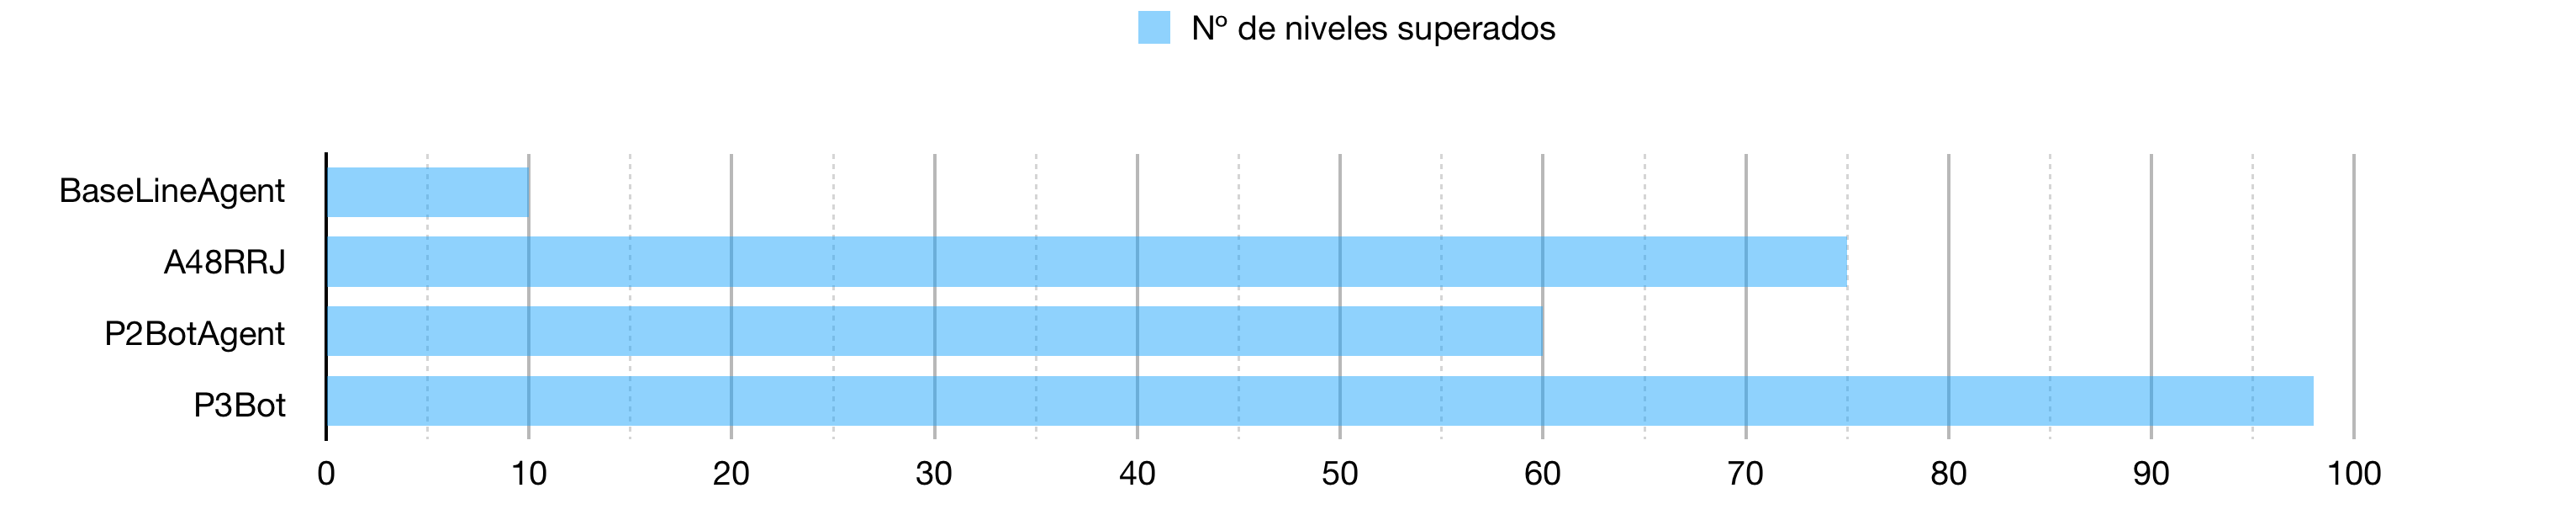
\includegraphics[width=170mm]{nivsup}
        %\caption{Total de niveles superados sobre 1000} % Titulo tabla en el indice
        \label{nivsup}
    \end{figure}
    \begin{figure}[h!] 
        \center
        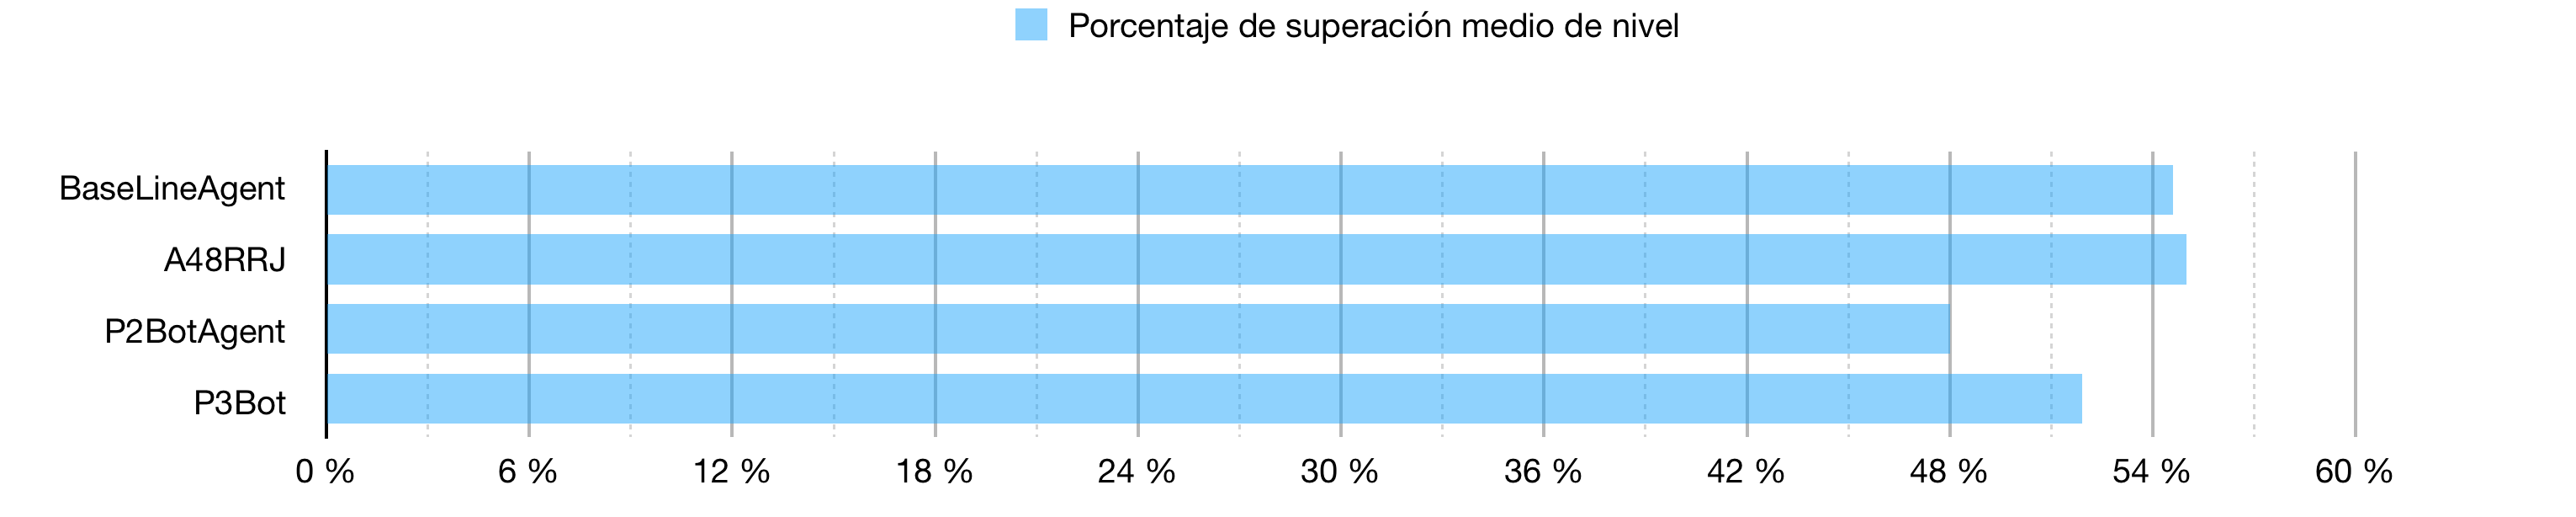
\includegraphics[width=170mm]{porcentaje}
        %\caption{ Porcentaje medio de la superación en cada nivel.} % Titulo tabla en el indice
        \label{porcentaje}
    \end{figure}
    \begin{figure}[h!] 
        \center
        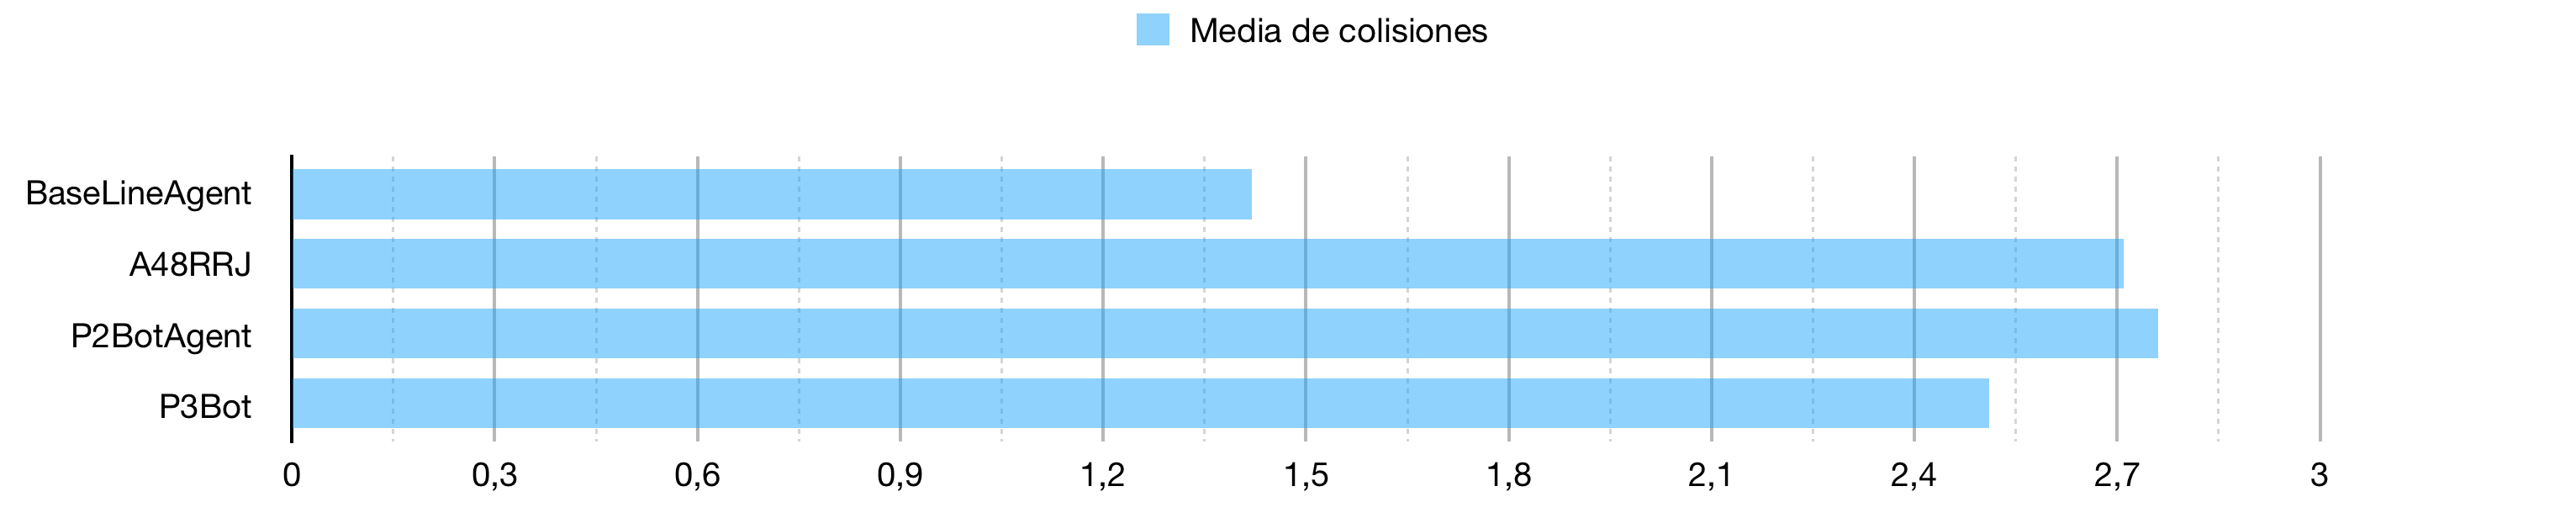
\includegraphics[width=170mm]{nivel}
        %\caption{ Media de colisiones con enemigo por nivel.} % Titulo tabla en el indice
        \label{nivel}
    \end{figure}
    \begin{figure}[h!]
        \center
        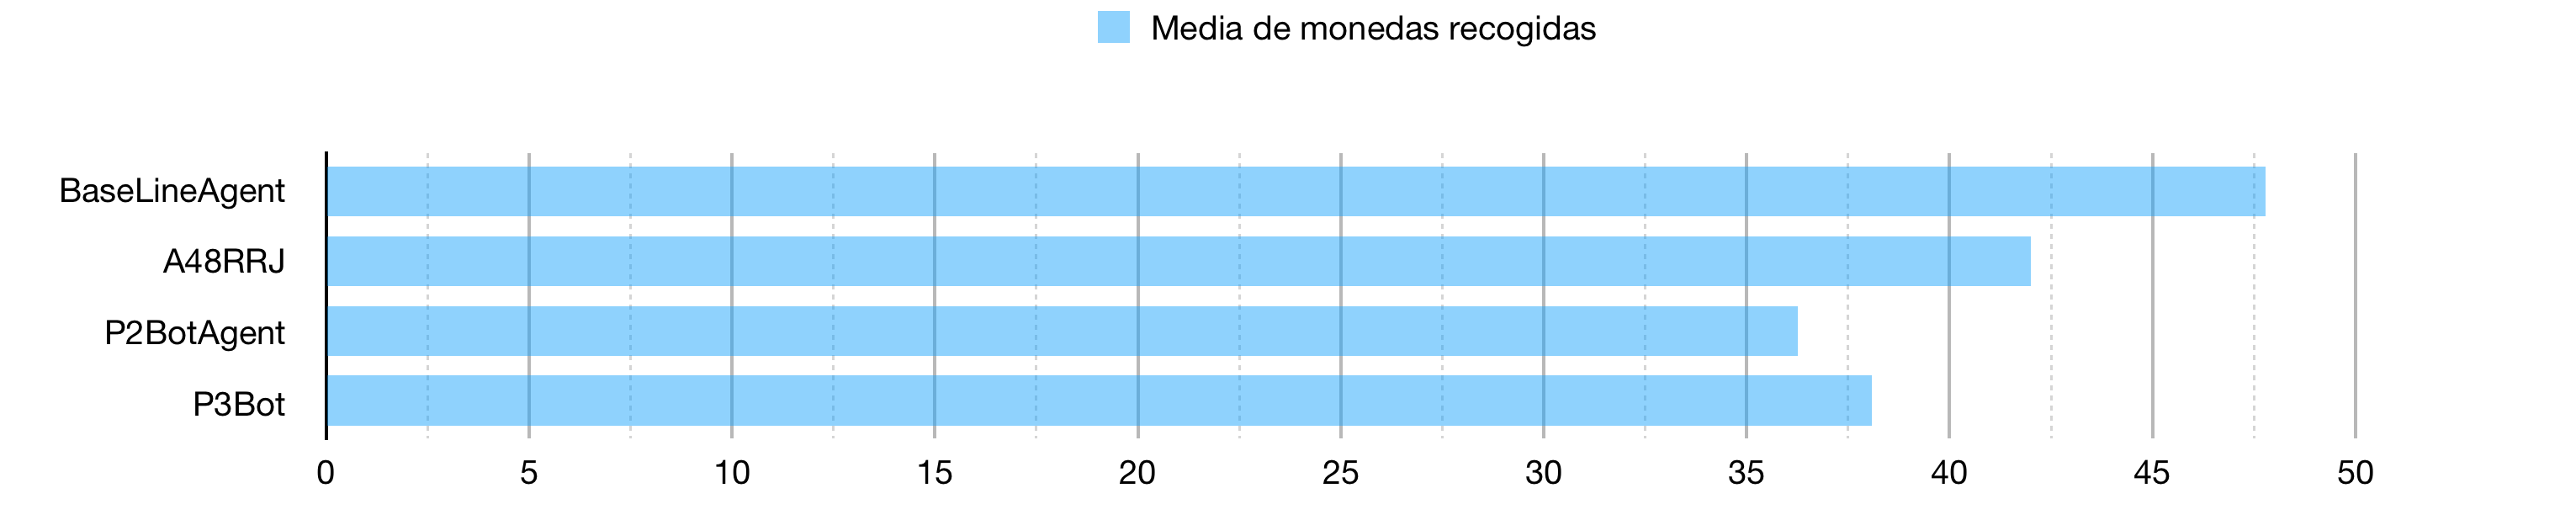
\includegraphics[width=170mm]{monedas}
        %\caption{ Media de monedas recogidas por nivel.} % Titulo tabla en el indice
        \label{monedas}
    \end{figure}
    \begin{figure}[h!]
        \center
        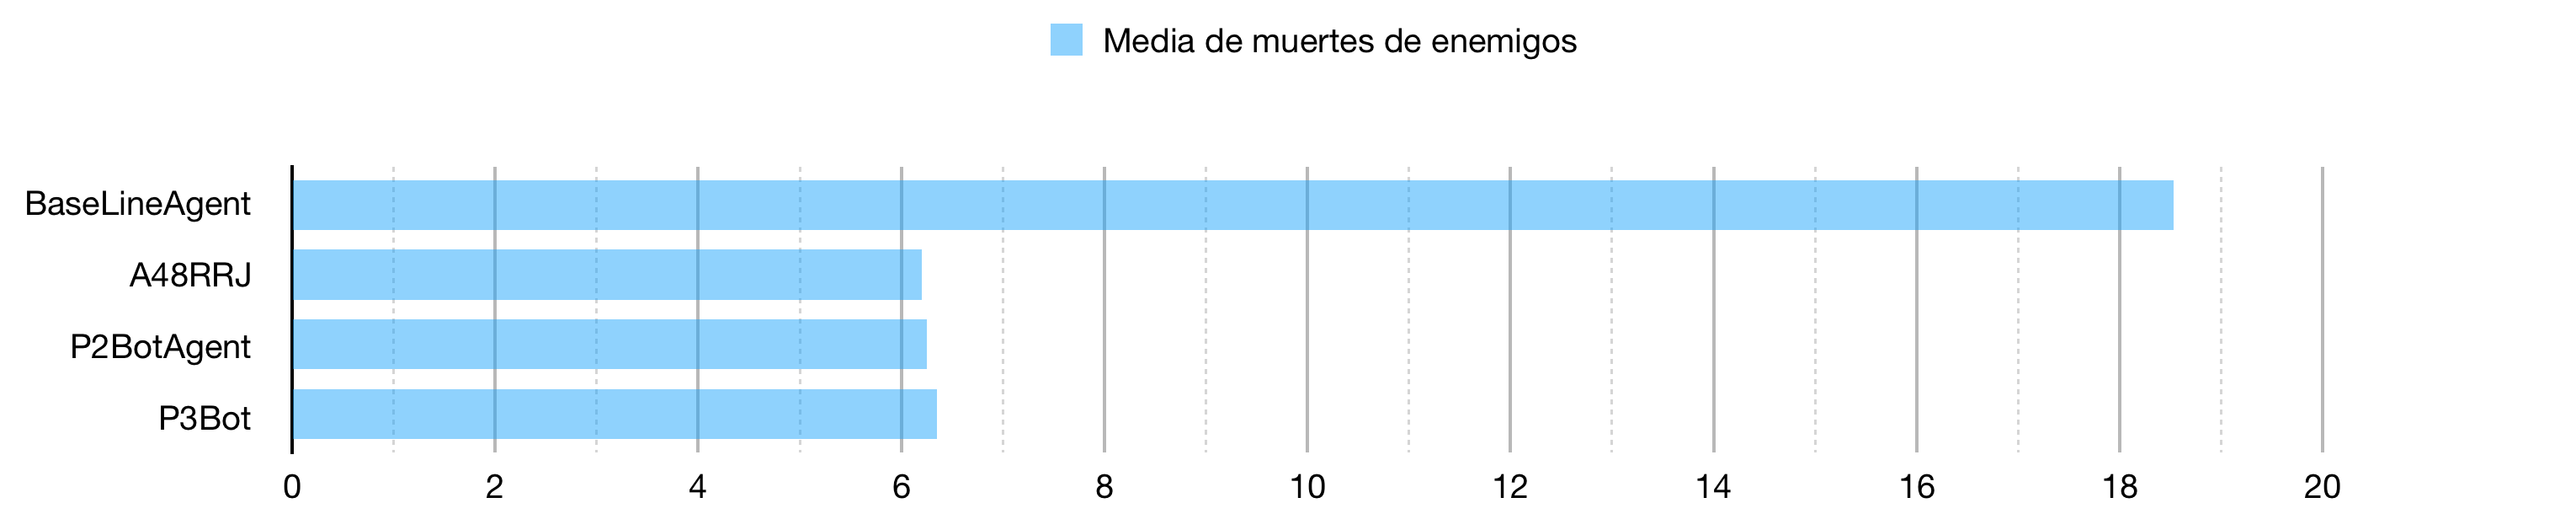
\includegraphics[width=170mm]{muertes}
        %\caption{ Media de muertes de enemigos por nivel.} % Titulo tabla en el indice
        \label{muertes}
    \end{figure}
    \clearpage

\section{Descripción del material entregado}\label{dme}
    \p{Junto a esta memoria, se entrega el siguiente material:}
    \begin{itemize}
        \item \textbf{estadísticas.sh:} script en bash utilizado para la captura de estadísticas, estudio y evaluación del agente para pequeños y grandes volúmenes de ejecuciones o niveles. Requiere como dependencia python 3. Su ejecución es la siguiente:
            \begin{center}
                \texttt{./estadísticas.sh\hspace{1em}<agente>\hspace{1em}<num\_niveles>}
            \end{center}
        \item ...
    \end{itemize}

\newpage
\section{Conclusiones}\label{c}
    \p{De la realización de un agente inteligente que utiliza \textit{Q-Learning} podemos concluir lo siguiente:}
    \begin{itemize}
        \item a
        \item b
        \item c
    \end{itemize}

\newpage
\section{Comentarios personales}\label{cp}
\p{Si bien la práctica ha sido entretenida y de una dificultad asequible, nos ha costado bastante obtener las situaciones en las que clasificar las instancias, así como determinar los pesos que aplicar a cada atributos en las funciones matemáticas euclídeas.}
\p{Si bien esto es una parte importante de la práctica y algunas decisiones se han tomado en base a criterios objetivos, como se ha detallado en esta memoria o en el código, mucho de estos pesos o clasificaciones se han calculado mediante prueba y error. Por eso, hubiésemos agradecido una guía, una clase, material o algún recurso que nos enseñara cómo calcular estos pesos de forma, si no óptima, al menos más razonada que el típico prueba y error.}
\p{Desarrollar estos apartados de la práctica mediante prueba y error nos ha resultado, además de improductivo y contraproducente (ya que no ha aportado conocimiento reseñable per se), una pérdida elevada de tiempo en un momento del cuatrimestre en el que la carga académica es muy elevada para todas las asignaturas.}

\end{document}